\documentclass[11pt,a4paper]{article}
\usepackage[left=1in,right=1in]{geometry}
\usepackage{fancyhdr}
\usepackage{graphicx}
\usepackage{amsmath}
\usepackage{booktabs}

\usepackage{capt-of}
\usepackage{tabu}

\usepackage[utf8]{inputenc} % allow utf-8 input
\usepackage[T1]{fontenc}    % use 8-bit T1 fonts
\usepackage{url}            % simple URL typesetting


\fancypagestyle{plain}{
  \fancyhf{}
  \fancyhead[L]{\sffamily University of Illinois Chicago}
  \fancyhead[R]{\sffamily Intro to Machine Learning, Fall 2023}
%   \fancyfoot[L]{\sffamily /department of computer science}
%   \fancyfoot[R]{\sffamily\bfseries\thepage}
  \renewcommand{\headrulewidth}{0.5pt}
  \renewcommand{\headrule}{\hbox to\headwidth{%
    \leaders\hrule height \headrulewidth\hfill}}
  \renewcommand{\footrulewidth}{0pt}% No footer rule
%   \renewcommand{\footrulewidth}{0.5pt}
}
% \fancypagestyle{plain}{\homework}



\title{Destiny Icon Classifier}
\author{Thomas Federmeyer}
\begin{document}
\date{} %leave this empty
% \pagestyle{myheader}
\maketitle

\section{Introduction}
The task for this project is to find a suitable model to classify the weapon and armor icons in the video game called Destiny. In this game there are many types of items, specifically weapons (hand cannons, swords, pulse rifles, etc…) and armor (helmets, chest plates, etc…) with every item being tagged with an  item class and a unique icon. The goal is to classify any random icon to the proper class label.

\subsection*{Known Issue:}

\begin{itemize}
  \item The provided icon set is fairly limited with less than 7,000 icons spread around 20 unique classes
  \item Some classes have more data than others, (Ex: Gauntlets: 1133 entries, Trace Rifles: 23 entries)
  \item Some images are special (exotic) and don't conform to the regular styles.
\end{itemize}

\subsection*{Findings}
Keeping these known issues in mind, after training on two different designs, the base Small Xception proved to have a great general out of box accuracy of  ≈74\% with four classes under 50\% and three classes with a 0\% classification rate. On the other hand my custom Simple Sodel model managed a lower ≈65\% accuracy and retained the four classes under 50\%, however the classes with a 0\% classification rate dropped to one. This finding help show that with the structure of the data, a simpler styled network could potentially yield stronger and more general results.

\section{Methods/Case Study}\label{sec:methods}
For this I have experimented with 2 different models. The first was a small form of Xception provided by keras, and the second was a custom model using a Sodel kernel. With the same data being provided to the each model.

\subsection*{Data:}
All the data that being used for training and testing is acquired from the public API
\footnote{Bungie API: \url{https://bungie-net.github.io}}
provided by Bungie the studio that developed the games Destiny(1 and 2). I will be using exclusively the icons that are related to a weapon (
Classes: 
Auto Rifle,
Combat Bow,
Fusion Rifle,
Grenade Launcher,
Hand Cannon,
Linear Fusion Rifle,
Machine Gun,
Pulse Rifle,
Rocket Launcher,
Scout Rifle,
Shotgun,
Sidearm,
Sniper Rifle,
Submachine Gun,
Sword, 
and Trace Rifle)
or armour (
Classes:
Chest Armor,
Gauntlets,
Leg Armor,
and Helmet
).
Some examples of these icons can be seen in Table \ref{table:data}.
Each of these Icons are 96x96 jpgs providing a consistent format among every image. During the training process the data will be split into a training (80\%)and validation (20\%) data set, randomly with a batch size of 64.



\begin{table}[!t]
\caption{Example of data}
\label{table:data}
\centering
\begin{tabu}to \textwidth {X[c]X[c]}
  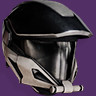
\includegraphics[width=45mm]{ml-report-template/Images/Helmet5.jpg}\captionof{figure}{Helmet} &
  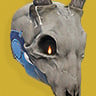
\includegraphics[width=45mm]{ml-report-template/Images/Helmet11.jpg}\captionof{figure}{Helmet} \\
  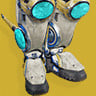
\includegraphics[width=45mm]{ml-report-template/Images/Leg Armor2.jpg}\captionof{figure}{Leg Armour} &
  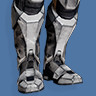
\includegraphics[width=45mm]{ml-report-template/Images/Leg Armor16.jpg}\captionof{figure}{Leg Armour} \\
  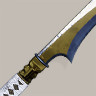
\includegraphics[width=45mm]{ml-report-template/Images/Sword5.jpg}\captionof{figure}{Sword}&
  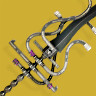
\includegraphics[width=45mm]{ml-report-template/Images/Sword30.jpg}\captionof{figure}{Sword} \\
   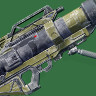
\includegraphics[width=45mm]{ml-report-template/Images/Rocket Launcher89.jpg}\captionof{figure}{Rocket Launcher}&
  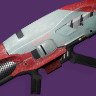
\includegraphics[width=45mm]{ml-report-template/Images/Rocket Launcher29.jpg}\captionof{figure}{Rocket Launcher} \\
\end{tabu}
\end{table}

\subsection*{Small Xception:}
For the initial test, I used the network that Keras has on their tutorial for image classification\footnote{link to the model: \url{https://keras.io/examples/vision/image_classification_from_scratch/}}. This implementation uses five main blocks of ReLU convolution max pooling each of which has increasing densities, and passing residuals from the beginning of the block to the end, and a final softmax function used to determine the probability for each class label (with the highest being used for classification). This slightly modified out of box solution is used to determine what a good benchmark to look at in terms of classification effectiveness is compared to  other networks. 

\subsection*{Custom Simple Sodel:}
The name Simple Sodel comes from the initial layers that's applied to the network before any other modifications. The point of this initial layer is to remove as much excess information that is not necessary for the classification network by applying edge detection using a Sodel \footnote{more information about Sodel: \url{https://en.wikipedia.org/wiki/Sobel_operator}} Kernel. In addition the model uses 2 main blocks of ReLU, convolution, max pooling layers and the same softmax function to determine the probability for each class label.  
\begin{center}
    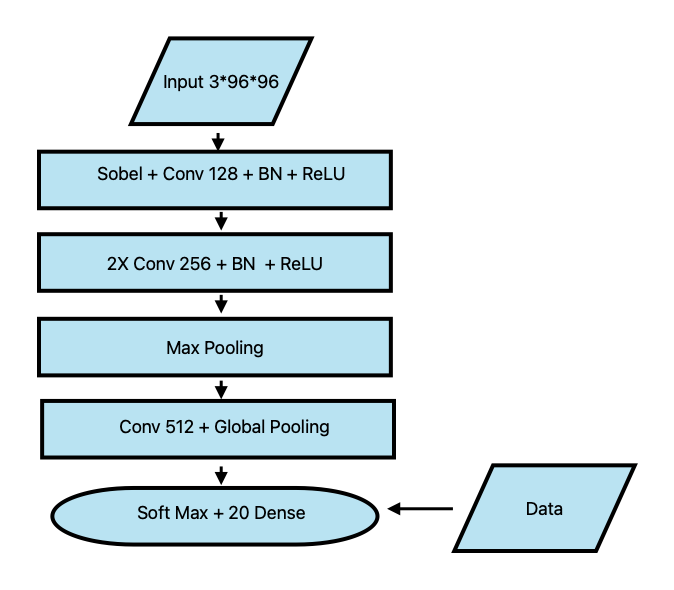
\includegraphics[width=45mm]{ml-report-template/Model.png}
\end{center}

\subsection*{Generalization:}
Both of these two models use the same concepts for generalization. They both use batch normalization in after each convolution layer, as well as a final dropout when converting to the final classification dense layer. Both of these are using together to proved a good generalization giving the unique nature of some images

\subsection*{Areas of Interest:}
Due to the large discrepancies in data-points for each classification label, instead of looking at the raw probability a more holistic view will be taken. This means a deeper look into the each class individually will be taken in account as well. these areas interest can be seen in comparison table (Table \ref{table:results})


\section{Results and Discussion\footnote{All the code an models can be found here: \url{https://github.com/ThomasFedermeyer/412_Bungie_Icons}
}} 

\subsection*{Results}

As mentioned in previous the results are broken into 3 sections:

\begin{itemize}
  \item The probability for getting a specific class correct.
  \item The average probability for getting a class correct.
  \[ 1/N\sum_{n=1}^{N} P(n)\] 
  \begin{center}
  \footrule{Number of classes = N}
  \end{center}
  \item The overall probability of any any given image correctly classified.
\end{itemize}

Each of these points of interest can be found in Table \ref{table:results}
, with the first 20 rows representing Probability for a singe class followed by average class correction then the overall probability. 

\begin{table}[h]
  \caption{Comparison of both models}
  \label{table:results}
  \vspace{0.1in}
    \centering
    \begin{tabular}{c| c|c}
        \toprule
         & Custom Simple Sodel & Small Xception \\
         \midrule
            Auto Rifle & 0.48148148148148145 &
0.7962962962962963 \\
            Chest Armor & 0.9091734786557675 &
0.9618528610354223 \\
            Combat Bow & 0.9836065573770492 &
1.0 \\
            Fusion Rifle & 0.456 &
0.992 \\
            Gauntlets & 0.999117387466902 & 
0.9814651368049426 \\
            Grenade Launcher & 0.6267605633802817 &
0.8661971830985915 \\
            Hand Cannon & 0.9615384615384616 &
0.9855769230769231 \\
            Helmet& 0.8633484162895928 &
0.9945701357466064 \\ 
            Leg Armor & 0.7990825688073394 &
0.9935779816513761 \\
            Linear Fusion Rifle& 0.13333333333333333 &
0.7333333333333333 \\
            Machine Gun& 0.9625 &
0.8375 \\
            Pulse Rifle& 0.30057803468208094 &
0.7225433526011561 \\
            Rocket Launcher& 0.8586956521739131 &
0.967391304347826 \\
            Scout Rifle& 0.5914634146341463 &
0.8292682926829268 \\
            Shotgun& 0.7085714285714285 &
0.8292682926829268 \\
            Sidearm& 0.33620689655172414 &
0.9568965517241379 \\
            Sniper Rifle& 0.7302631578947368 &
0.0 \\
            Submachine Gun& 0.528169014084507 &
0.0 \\
            Sword& 0.7441860465116279 &
0.0 \\
            Trace Rifle& 0.0 &
0.2608695652173913 \\
            Class Average& 0.6487037946717187 &
0.7391098030237035 \\
            Total Accuracy& 0.8103529411764706 &
0.8972549019607843 \\
      \bottomrule
    \end{tabular}
\end{table}

\subsection*{Discussion}

Looking at the data collected, the base Small Xception model comes across as a clear winner with an total accuracy $\approx$8\% greater than its Simple Sodel counter part. This trend is continued when looking at the average class accuracy with $\approx$+9\% difference this time. 

However the overall effectiveness is not the only axis that important in this project, its also important to look at the similarities and differences. With an initial glance over the Table \ref{table:results} it might be surprising that with a relatively high total accuracy ($\approx$81\% and $\approx$90\% respectively)that the class average is much lower ($\approx$65\% and $\approx$74\% respectively), however with the data that's used during training and comparison its not as much of a surprise. Its no coincidence that the classes with the highest classification probability (
Chest Armor,
Gauntlets,
Leg Armor,
and Helmet
)
, are also the classes that have 1000+ images. While the classes (
Sword
and Trace Rifle
)
that have limited data (85 and 22 respectively) are among the lowest.

The result that's truly shocking is the amount of classes with a 0\% classification probability in the Small Xception model. While it it expected for classes that have limited input data to have substantially lower probability, having three classes that with 0\% is quite interesting. Contrary to this the Simple Sodel Model reduces the 0\% rates to only one class. While this can be seen as model being too general and 'not effective', looking further at general trends say different. Classes with under 50\% for both of the models remain consistent at 4 (albeit different). 

With these interesting results, we can see how a model like the Custom Simple Sodel can provide a stronger classification if it was tailored more towards the data it was given. Along with how the strong over all effectiveness can also have underlying problems in its other results.


\section{Conclusion}
Overall This project has provide 3 major axes when it comes to learning, general findings, general TensorFlow/Keras knowledge, and data/model importance. 

\subsection*{General Findings}

The finding that stood out as important where from the model comparisons. It was interesting to study the difference in output and accuracy's of the two models. With the most interesting lesson being how a worse overall model can produce some more general outcomes that could be seen as better and a stronger classier. For project like this, given the style of data provided, a smaller model like the Custom Simple Sodel tailored more towards the situation could provide a better result.

\subsection*{TensorFlow/Keras}

With this project being open ended with no started code, it allowed me to explore more concepts in the TensorFlow library. With most of the class programming assignments focusing on the math or concepts behind the models. This Project on the other had, has enabled me to learn a more holistic approach staring from the bottom up. This has included collection and loading data, creating a model, testing a models effectiveness, and comparing two different models.


\subsection*{Data/Model Importance}

Due to the interesting and limited data available for this project, it has taught me the importance around data and how it can effect different models effectiveness. The specific lesson learned is the importance of balanced data. This is highly seen in the discrepancy in total accuracy and average class accuracy.

\subsection*{Reference}
%you can use the bibliography citation if you want
[1] S. Sodha, “An implementation of sobel edge detection” Rhea, \url{https://www.projectrhea.org/rhea/index.php/An_Implementation_of_Sobel_Edge_Detection} (accessed Dec. 3, 2023). \newline
[2] drum\_stick, “How to construct a Sobel filter for kernel initialization in input layer for images of size 128x128x3?,” Stack Overflow, \url{https://stackoverflow.com/questions/61983606/how-to-construct-a-sobel-filter-for-kernel-initialization-in-input-layer-for-ima} (accessed Dec. 20, 2023). \newline
[3] K. Team, “Keras documentation: Image Classification From Scratch,” Keras, \url{https://keras.io/examples/vision/image_classification_from_scratch/} (accessed Nov. 24, 2023). 
\end{document}
